\documentclass[12pt,a4paper]{article}

\usepackage[utf8]{inputenc}
\usepackage{amsmath, amssymb, amsthm}
\usepackage{graphicx}
\usepackage{float}
\usepackage{booktabs}
\usepackage{tabularx}
\usepackage{siunitx}
\usepackage{hyperref}
\usepackage{bm}
\usepackage{natbib} % or biblatex if you prefer
\bibliographystyle{apa} % set APA style
\usepackage{multirow}

\title{Time Series Clustering Using Simulated Data}
\author{Rasika Dilhani}
\date{\today}


\begin{document}
	\maketitle
	
\section{Introduction}
Time series analysis provides a framework for characterizing the structural properties of data and its random variation. In this study, we conduct a simulation experiment to examine the features of ordinal patterns within ARMA (Autoregressive Moving Average) processes. To do this, we use simulated data, also known as synthetic series, which are generated from specified time series models. Simulation plays a main role in time series research, as it facilitates the assessment of statistical properties, the construction of confidence intervals for model parameters, and the exploration of potential future scenarios. Furthermore, simulation methods are computationally accessible,  as most standard statistical distributions can be generated directly through established algorithms. To explore the features of ordinal patterns, we replicate the experiment under two different sample sizes. The aim was to investigate how different ARMA parameter settings influence the stochastic properties of the resulting time series data, particularly in terms of entropy, complexity, and other statistical features.

	
\section{ARMA model}
In this study, simulated datasets are generated for clustering time series using ordinal patterns. The base random model for sampling is the normal distribution: $\bm X=(X_1,X_2,\dots,X_n)$, with $X_i \sim N(\mu, \sigma^2)$. Here, the mean parameter varies as $\mu \in \{-1, 0, 1\}$. For investigating more complex dynamics, simulated time series are constructed using autoregressive moving average (ARMA) models, a central class of models for representing stationary processes.

\subsection{The Backward Shift (Lag) Operator}

The backward shift (or lag) operator $\mathbf{B}$ is defined as $\mathbf{B} x_t = x_{t-1}$. By repeated application, this yields $\mathbf{B}^n x_t = x_{t-n}$. This compact notation is fundamental in expressing ARMA models and related difference equations.

\subsection{ARMA Model Specification}

Let $\{x_t\}$ denote a real-valued time series. An ARMA($p,q$) process can be written as:
\begin{equation}
	x_t = \alpha_1 x_{t-1} + \alpha_2 x_{t-2} + \dots + \alpha_p x_{t-p} + w_t + \beta_1 w_{t-1} + \beta_2 w_{t-2} + \dots + \beta_q w_{t-q},
	\label{eq:arma}
\end{equation}
where $\{w_t\}$ is a white noise sequence.

Using the lag operator, the above model can be expressed more compactly as:
\begin{equation}
	\theta_p(\mathbf{B}) x_t = \phi_q(\mathbf{B}) w_t,
	\label{eq:arma_polynomial}
\end{equation}
where $\theta_p(\mathbf{B}) = 1 - \alpha_1 \mathbf{B} - \alpha_2 \mathbf{B}^2 - \cdots - \alpha_p \mathbf{B}^p$ and $\phi_q(\mathbf{B}) = 1 + \beta_1 \mathbf{B} + \cdots + \beta_q \mathbf{B}^q$.

\subsection{Parameter Constraint for ARMA model}
In an ARMA model, the constraints are about two things. The AR part must satisfy stationarity, meaning the series has constant mean and variance over time. The MA part must satisfy invertibility, meaning the model can be written in terms of past observations. These rules apply to ARMA($p,q$) models. 

\begin{itemize}
\item \textbf{AR part (stationarity):}
	\begin{itemize}
		\item AR coefficients ($\phi_i$) must satisfy stationarity.
		\item Roots of the AR polynomial must lie outside the unit circle.
		\item Conditions:
		\begin{itemize}
			\item \textbf{AR(1):} $-1 < \phi_1 < 1$.
			\item \textbf{AR(2):} all three must hold:
			\begin{itemize}
				\item $-1 < \phi_2 < 1$
				\item $\phi_2 + \phi_1 < 1$
				\item $\phi_2 - \phi_1 < 1$
			\end{itemize}
			\item \textbf{AR($p \geq 3$):} all roots of
			\[
			1 - \phi_1 x - \phi_2 x^2 - \dots - \phi_p x^p = 0
			\]
			must lie outside the unit circle.
		\end{itemize}
	\end{itemize}
	
\item \textbf{MA part (invertibility):}
	\begin{itemize}
		\item MA coefficients ($\theta_j$) must ensure invertibility.
		\item Roots of the MA polynomial must also lie outside the unit circle.
		\item Conditions:
		\begin{itemize}
			\item \textbf{MA(1):} $-1 < \theta_1 < 1$.
			\item \textbf{MA(2):} all three must hold:
			\begin{itemize}
				\item $-1 < \theta_2 < 1$
				\item $\theta_2 + \theta_1 < 1$
				\item $\theta_2 - \theta_1 < 1$
			\end{itemize}
		\end{itemize}
	\end{itemize}
\end{itemize}

If these constraints are violated, the ARMA model is not stationary or invertible, and is invalid for forecasting or inference.


\section{Parameter Settings and Data Generation}

To systematically analyze time series structure via entropy and complexity, we define a comprehensive grid of ARMA model configurations. The following models and coefficient settings are considered:

\begin{table}[H]
	\centering
	\begin{tabular}{llrrrr}
		\toprule
		\textbf{Type} & \textbf{Model} & $\alpha_1$ & $\alpha_2$ & $\beta_1$ & $\beta_2$ \\
		\midrule
		\multirow{4}[2]{*}{$\mathrm{AR}(1)$}      & $\mathrm{AR}(1)_{\textrm{M}_1}$  & $0.8$   &      &      &      \\
		& $\mathrm{AR}(1)_{\textrm{M}_2}$   & $0.1$   &      &      &      \\
		& $\mathrm{AR}(1)_{\textrm{M}_3}$   & $-0.8$  &      &      &      \\
		& $\mathrm{AR}(1)_{\textrm{M}_4}$   & $-0.1$  &      &      &      \\
		\midrule
		\multirow{4}[2]{*}{$\mathrm{AR}(2)$}      & $\mathrm{AR}(2)_{\textrm{M}_1}$   & $0.1$   & $0.8$  &      &      \\
		& $\mathrm{AR}(2)_{\textrm{M}_2}$  & $-0.8$  & $0.1$  &      &      \\
		& $\mathrm{AR}(2)_{\textrm{M}_3}$  & $0.1$   & $-0.8$ &      &      \\
		& $\mathrm{AR}(2)_{\textrm{M}_4}$  & $-0.8$  & $-0.1$ &      &      \\
		\midrule
		\multirow{4}[2]{*}{	$\mathrm{MA}(1)$}      & $\mathrm{MA}(1)_{\textrm{M}_1}$ &       &      & $0.8$  &      \\
		& $\mathrm{MA}(1)_{\textrm{M}_2}$  &       &      & $0.1$  &      \\
		& $\mathrm{MA}(1)_{\textrm{M}_3}$  &       &      & $-0.8$ &      \\
		& $\mathrm{MA}(1)_{\textrm{M}_4}$  &       &      & $-0.1$ &      \\
		\midrule
		\multirow{4}[2]{*}{$\mathrm{MA}(2)$}      & $\mathrm{MA}(2)_{\textrm{M}_1}$  &       &      & $0.1$  & $0.8$  \\
		& $\mathrm{MA}(2)_{\textrm{M}_2}$  &       &      & $-0.8$ & $0.1$  \\
		& $\mathrm{MA}(2)_{\textrm{M}_3}$  &       &      & $0.1$  & $-0.8$ \\
		& $\mathrm{MA}(2)_{\textrm{M}_4}$  &       &      & $-0.8$ & $-0.1$ \\
		\midrule
		\multirow{4}[2]{*}{$\mathrm{ARMA}(1,1)$}  & $\mathrm{ARMA}(1,1)_{\textrm{M}_1}$ & $0.8$ &      & $0.8$  &      \\
		& $\mathrm{ARMA}(1,1)_{\textrm{M}_2}$ & $0.1$ &      & $0.1$  &      \\
		& $\mathrm{ARMA}(1,1)_{\textrm{M}_3}$ & $-0.8$ &     & $-0.8$ &      \\
		& $\mathrm{ARMA}(1,1)_{\textrm{M}_4}$ & $-0.1$ &     & $-0.1$ &      \\
		\midrule
		\multirow{4}[2]{*}{$\mathrm{ARMA}(2,2)$}  & $\mathrm{ARMA}(2,2)_{\textrm{M}_1}$ & $0.1$ & $0.8$  & $0.1$  & $0.8$  \\
		& $\mathrm{ARMA}(2,2)_{\textrm{M}_2}$ & $-0.8$ & $0.1$ & $-0.8$ & $0.1$  \\
		& $\mathrm{ARMA}(2,2)_{\textrm{M}_3}$ & $0.1$ & $-0.8$ & $0.1$  & $-0.8$ \\
		& $\mathrm{ARMA}(2,2)_{\textrm{M}_4}$ & $-0.8$ & $-0.1$ & $-0.8$ & $-0.1$ \\
		\bottomrule
	\end{tabular}
		\caption{Models and parameter sets for AR(1), AR(2), MA(1), MA(2), ARMA(1,1), and ARMA(2,2). Empty cells indicate omitted parameters.}
	\end{table}


For each model type and specified parameterization:
\begin{itemize}
	\item Embedding dimension $D=3$ is used for ordinal pattern analysis.
	\item Sample sizes: $n \in \{500, 1000\}$.
	\item For each parameter configuration and each sample size, $R=100$ independent time series are simulated.
	\begin{itemize}
	\item For every time series, both permutation entropy ($H$) and statistical complexity ($C$) are computed.
	\item Each set of $(H, C)$ results is visualized: the $(H, C)$  pairs are plotted in the entropy-complexity plane, incorporating boundary curves and using axis splits suitable to each model and time series length.
	\end{itemize}
	\item For further insight, density plots grouped by sample size illustrate the distribution of points.
	\item For each model, four subplots (corresponding to four specific parameter combinations) are combined into one grid, yielding six grids (one per model type) for a total of $6 \times 4$ subplots.
\end{itemize}

The simulation design provides systematic coverage of AR, MA, and ARMA structures, supporting robust clustering analysis of ordinal pattern features in both short ($n=500$) and moderate ($n=1000$) time series settings. Visualization strategies enable both direct comparisons between parameterizations and analysis of overall model class behavior in the entropy-complexity space.

For a more detailed investigation of the results, each process type was analyzed separately with respect to the AR, MA, and ARMA model structures.


\section{Results}

To evaluate the effectiveness of ordinal pattern features for time series analysis, simulation experiments were conducted with ARMA processes across a comprehensive grid of parameters. Specifically, the autoregressive (AR) and moving average (MA) coefficients were varied over the sets:
\[
\text{AR} \in \{-0.8,\ -0.1,\ 0.8,\ 0.1 \}
\]
\[
\text{MA} \in \{-0.8,\ -0.1,\ 0.8,\ 0.1 \}
\]
For each combination of AR and MA parameters, a time series was simulated and analyzed using ordinal patterns. The simulation loop systematically covered all grid points, ensuring a variety of dynamic behaviors and noise structures.

\subsection{Summary Statistics}

\begin{table}[H]
	\centering
	\caption{Summary Statistics for AR1, MA1, ARMA11 Models}
	\begin{tabular}{lcccccc}
		\toprule
		Model & AR1 Mean & AR1 SD & MA1 Mean & MA1 SD & ARMA11 Mean & ARMA11 SD \\
		\midrule
		M1    & 0.0186   & 1.66   & 0.0341   & 1.30   & -0.1553     & 3.02      \\
		M2    & -0.0437  & 0.99   & -0.0423  & 0.98   & -0.0364     & 1.03      \\
		M3    & -0.0132  & 1.52   & -0.0043  & 1.26   & -0.0031     & 2.81      \\
		M4    & -0.0799  & 1.01   & -0.0735  & 0.98   & 0.0108      & 1.04      \\
		\bottomrule
	\end{tabular}
\end{table}

\begin{table}[H]
	\centering
	\caption{Summary Statistics for AR2, MA2, ARMA22 Models}
	\begin{tabular}{lcccccc}
		\toprule
		Model & AR2 Mean & AR2 SD & MA2 Mean & MA2 SD & ARMA22 Mean & ARMA22 SD \\
		\midrule
		M1    & -0.4445  & 2.05   & -0.0204  & 1.32   & 0.7426      & 3.34      \\
		M2    & -0.0161  & 2.03   & -0.0048  & 1.28   & -0.0047     & 3.91      \\
		M3    & -0.0322  & 1.72   & -0.0098  & 1.26   & -0.0075     & 2.63      \\
		M4    & 0.0158   & 1.51   & 0.0012   & 1.31   & -0.0038     & 2.33      \\
		\bottomrule
	\end{tabular}
\end{table}

\subsection{Time Series Visualization}
Visual inspection of time series plots shows expected differences:
\begin{itemize}
	\item \textbf{AR Models:} Display persistent oscillatory patterns, with some models M1 and M3 exhibiting greater volatility due to higher AR coefficients. Further, the summary statistics reinforce this, the larger standard deviation is observed for higher order or more persistent model ($\mathrm{AR}(2)_{\textrm{M}_1}$).  
	\item \textbf{MA Models:} Display short persistent deviation, generally lower variance compare to AR models.
	\item \textbf{ARMA Models:} Combine AR and MA dynamics, showing both strong persistence and sudden volatility spikes. Summary statistics capture $\mathrm{ARMA}(2,2)_{\textrm{M}_1}$ has both the highest standard deviation and the widest range among all models.  
\end{itemize}

\subsection{Ordinal Pattern Clustering}
Ordinal pattern clustering, guided by entropy-complexity features, effectively separates these time series models:
\begin{itemize}
	\item AR models form clusters characterized by low entropy, moderate complexity.
	\item MA models cluster around higher entropy and low complexity.
	\item ARMA models typically present higher complexity and greater dispersion, reflecting hybrid dynamics.
\end{itemize}

Figures~\ref{fig:TS AR(1)} to~\ref{fig:TS ARMA(22)}  display time series plots derived from simulated data, covering diverse AR and MA parameter combinations and sample sizes.  %$\mathrm{AR}(1)$ to $\mathrm{ARMA}(2,2)$ 

\begin{figure}[H]
		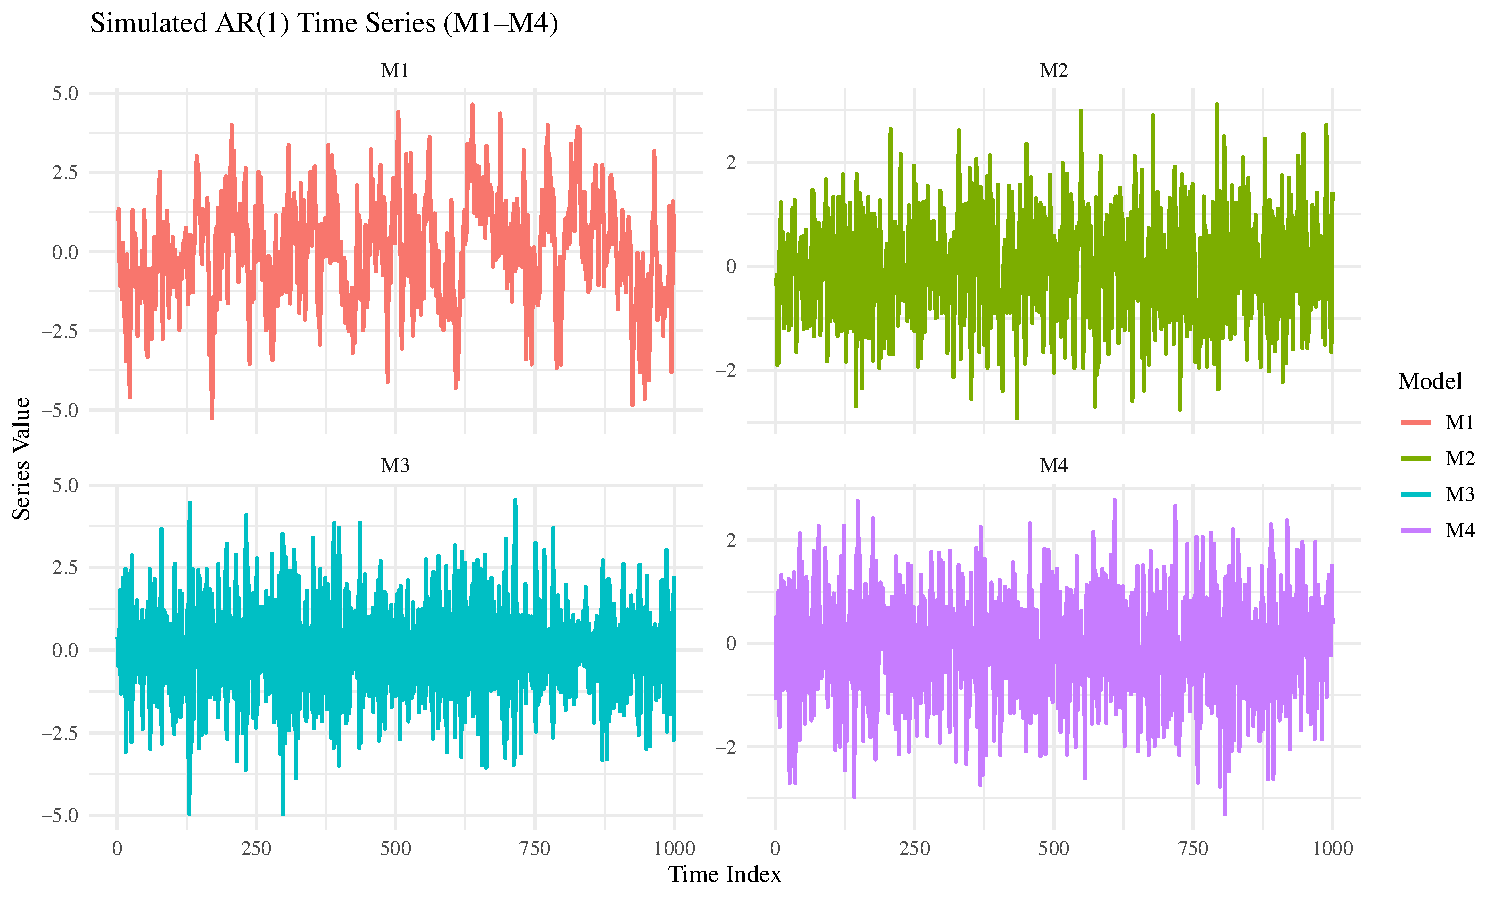
\includegraphics[width=0.9 \textwidth]{ar1_time_series_plot}
		\caption{Time series for $\mathrm{AR}(1)$ model}
		\label{fig:TS AR(1)}
\end{figure}	

\begin{figure}[H]
	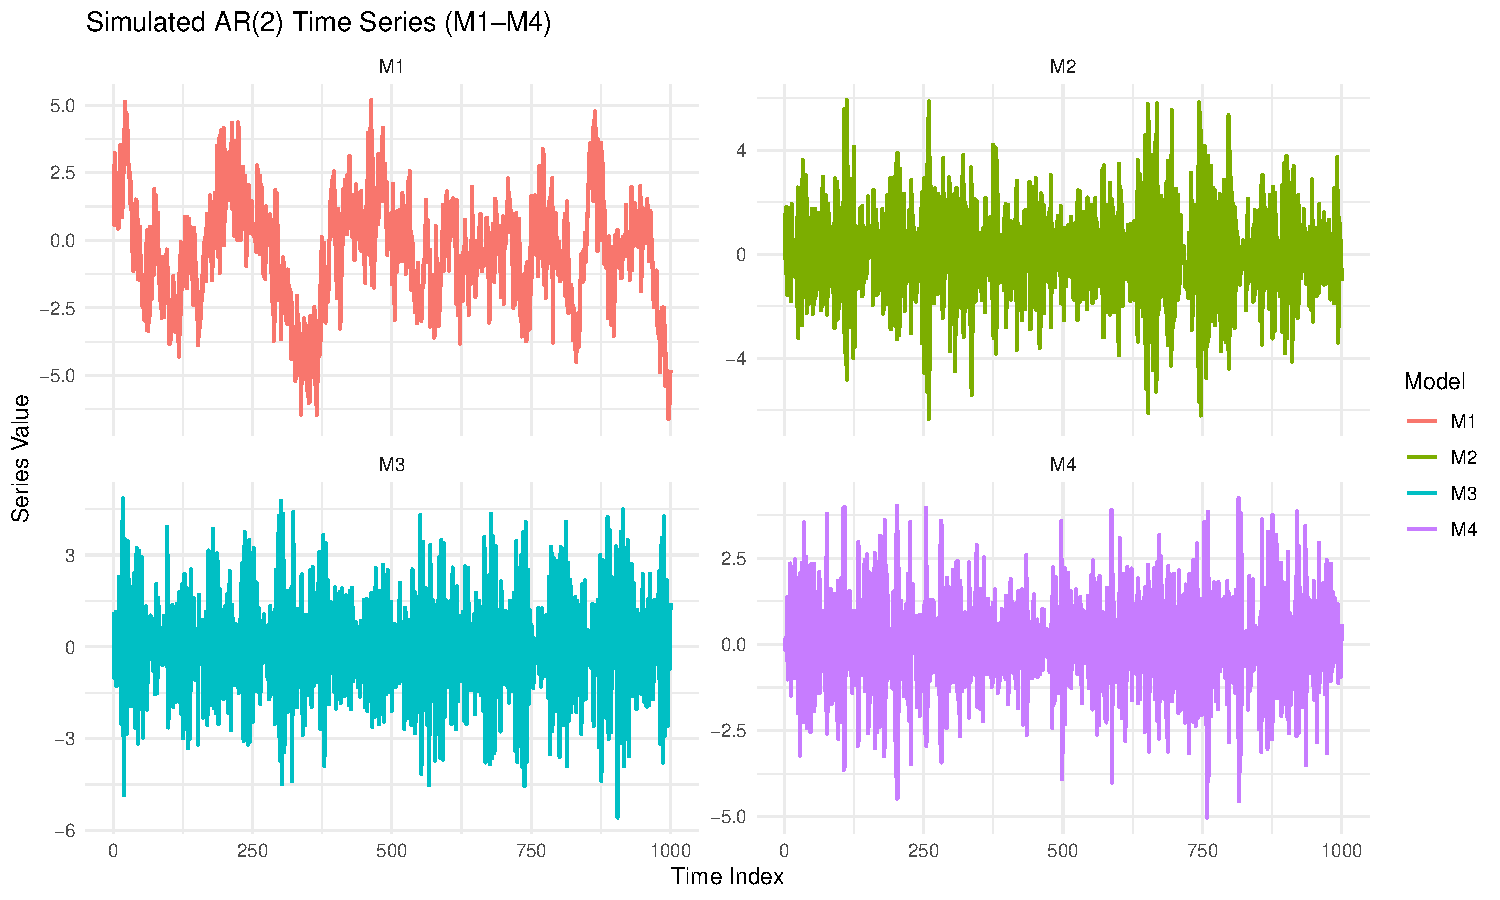
\includegraphics[width=0.9 \textwidth]{ar2_time_series_plot}
	\caption{Time series for $\mathrm{AR}(2)$ model}
	\label{fig:TS AR(2)}
\end{figure}	

\begin{figure}[H]
	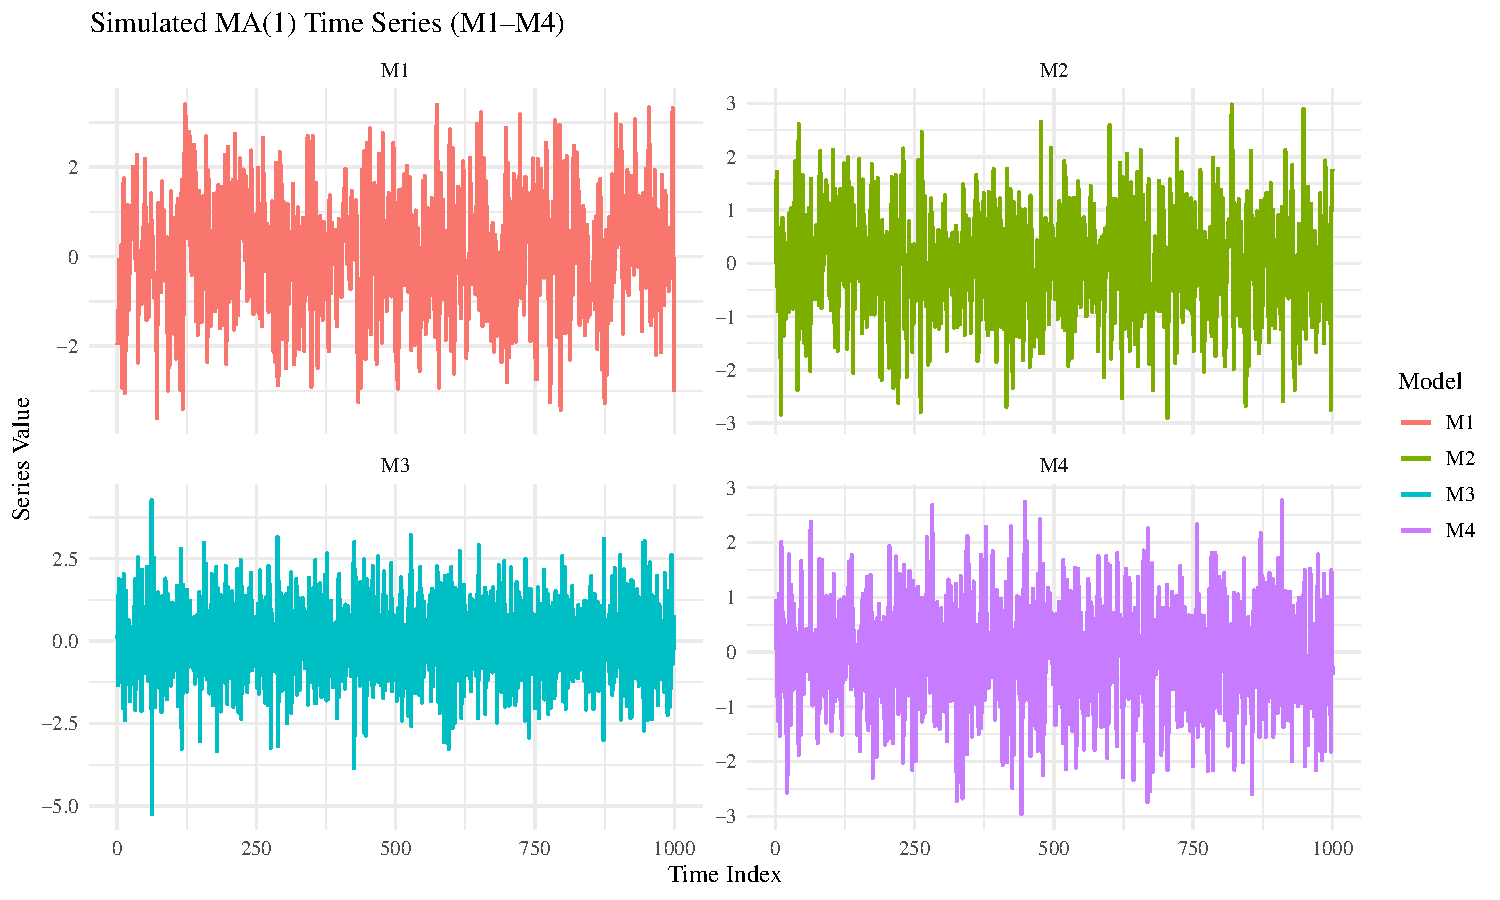
\includegraphics[width=0.9 \textwidth]{ma1_time_series_plot}
	\caption{Time series for $\mathrm{MA}(1)$ model}
	\label{fig:TS MA(1)}
\end{figure}	

\begin{figure}[H]
	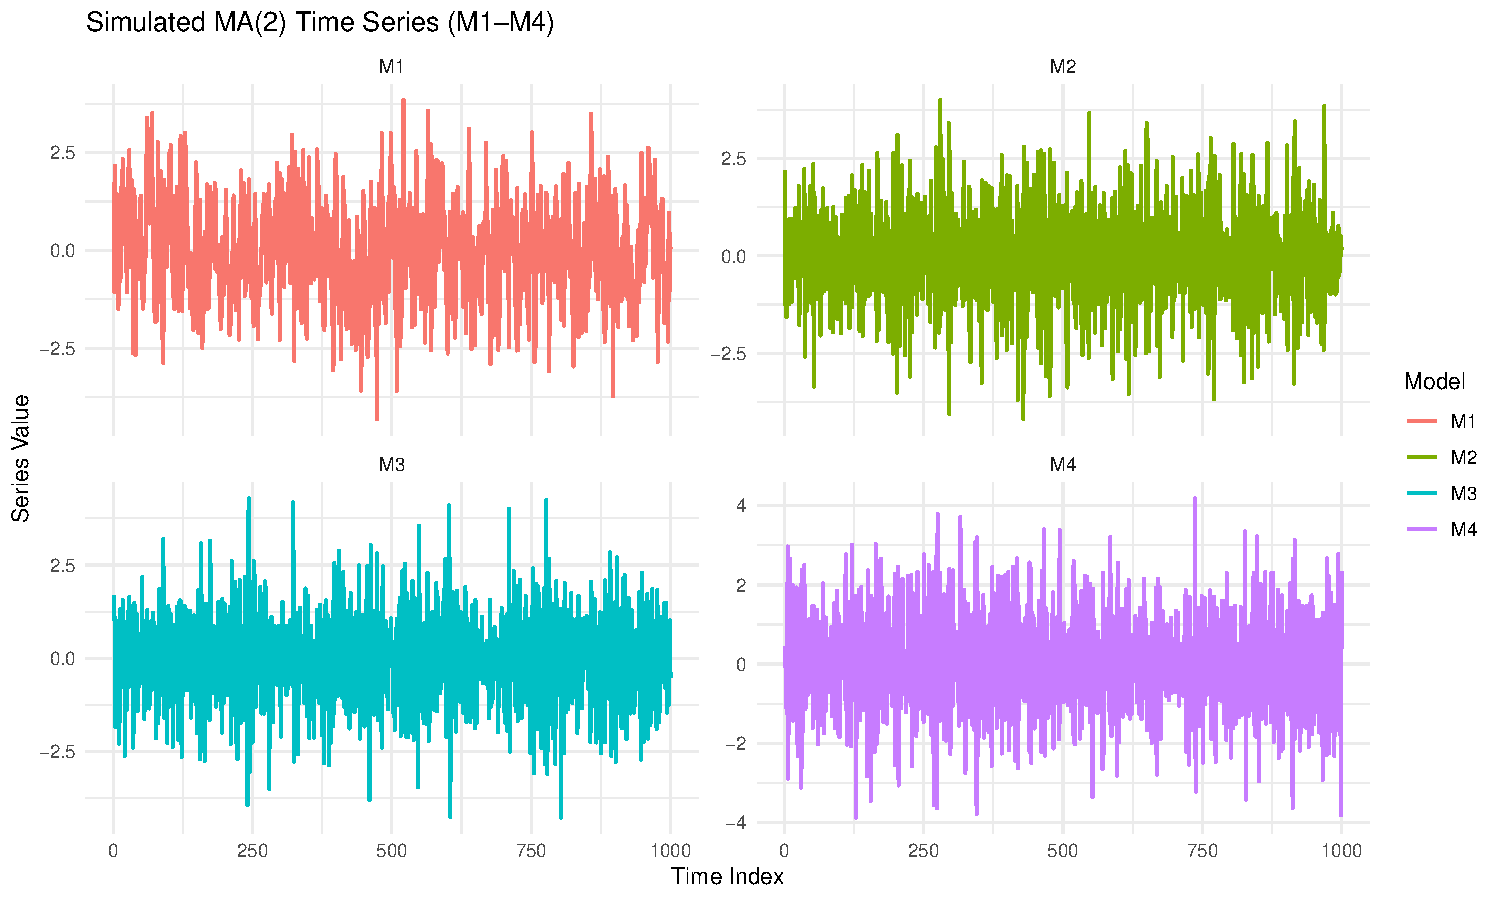
\includegraphics[width=0.9 \textwidth]{ma2_time_series_plot}
	\caption{Time series for $\mathrm{MA}(2)$ model}
	\label{fig:TS MA(2)}
\end{figure}	

\begin{figure}[H]
	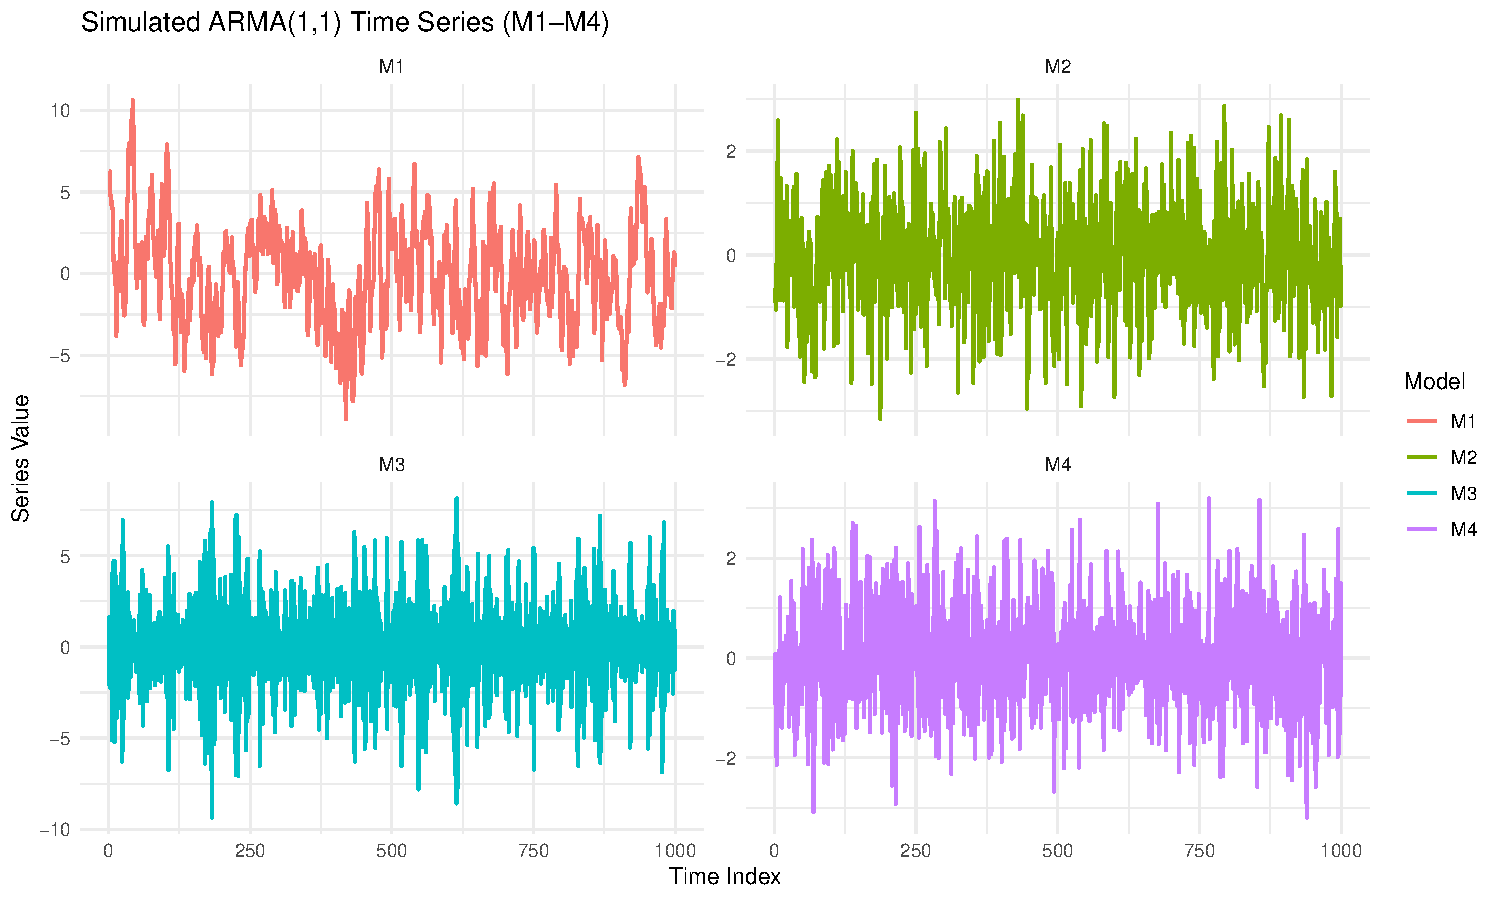
\includegraphics[width=0.9 \textwidth]{arma11_time_series_plot}
	\caption{Time series for $\mathrm{ARMA}(1,1)$ model}
	\label{fig:TS ARMA(11)}
\end{figure}	

\begin{figure}[H]
	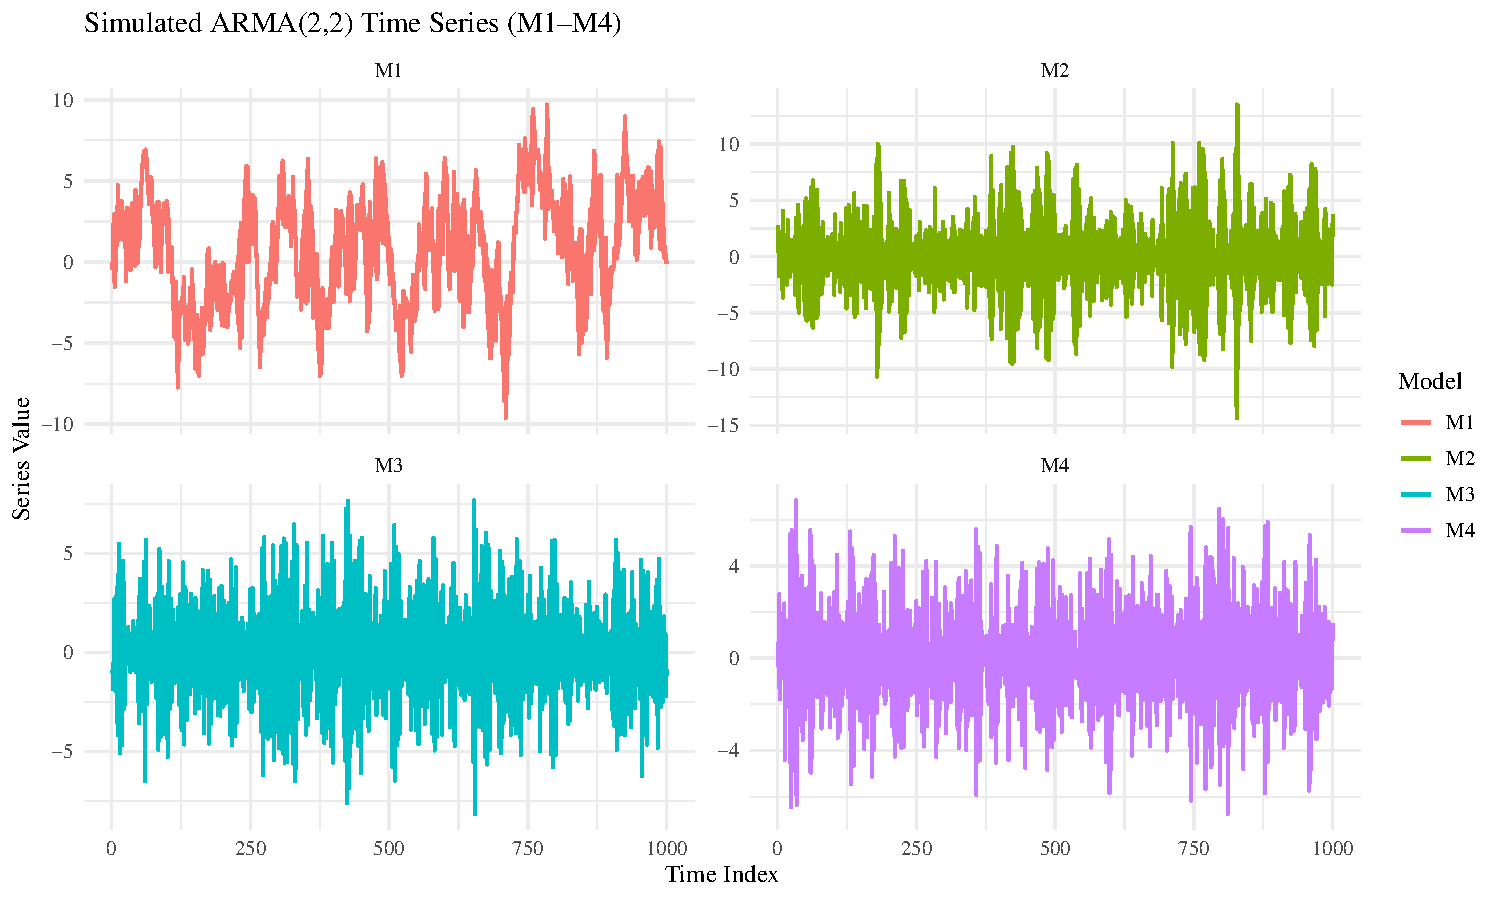
\includegraphics[width=0.9 \textwidth]{arma22_time_series_plot}
	\caption{Time series for $\mathrm{ARMA}(2,2)$ model}
	\label{fig:TS ARMA(22)}
\end{figure}	

%\begin{figure}[H]
%	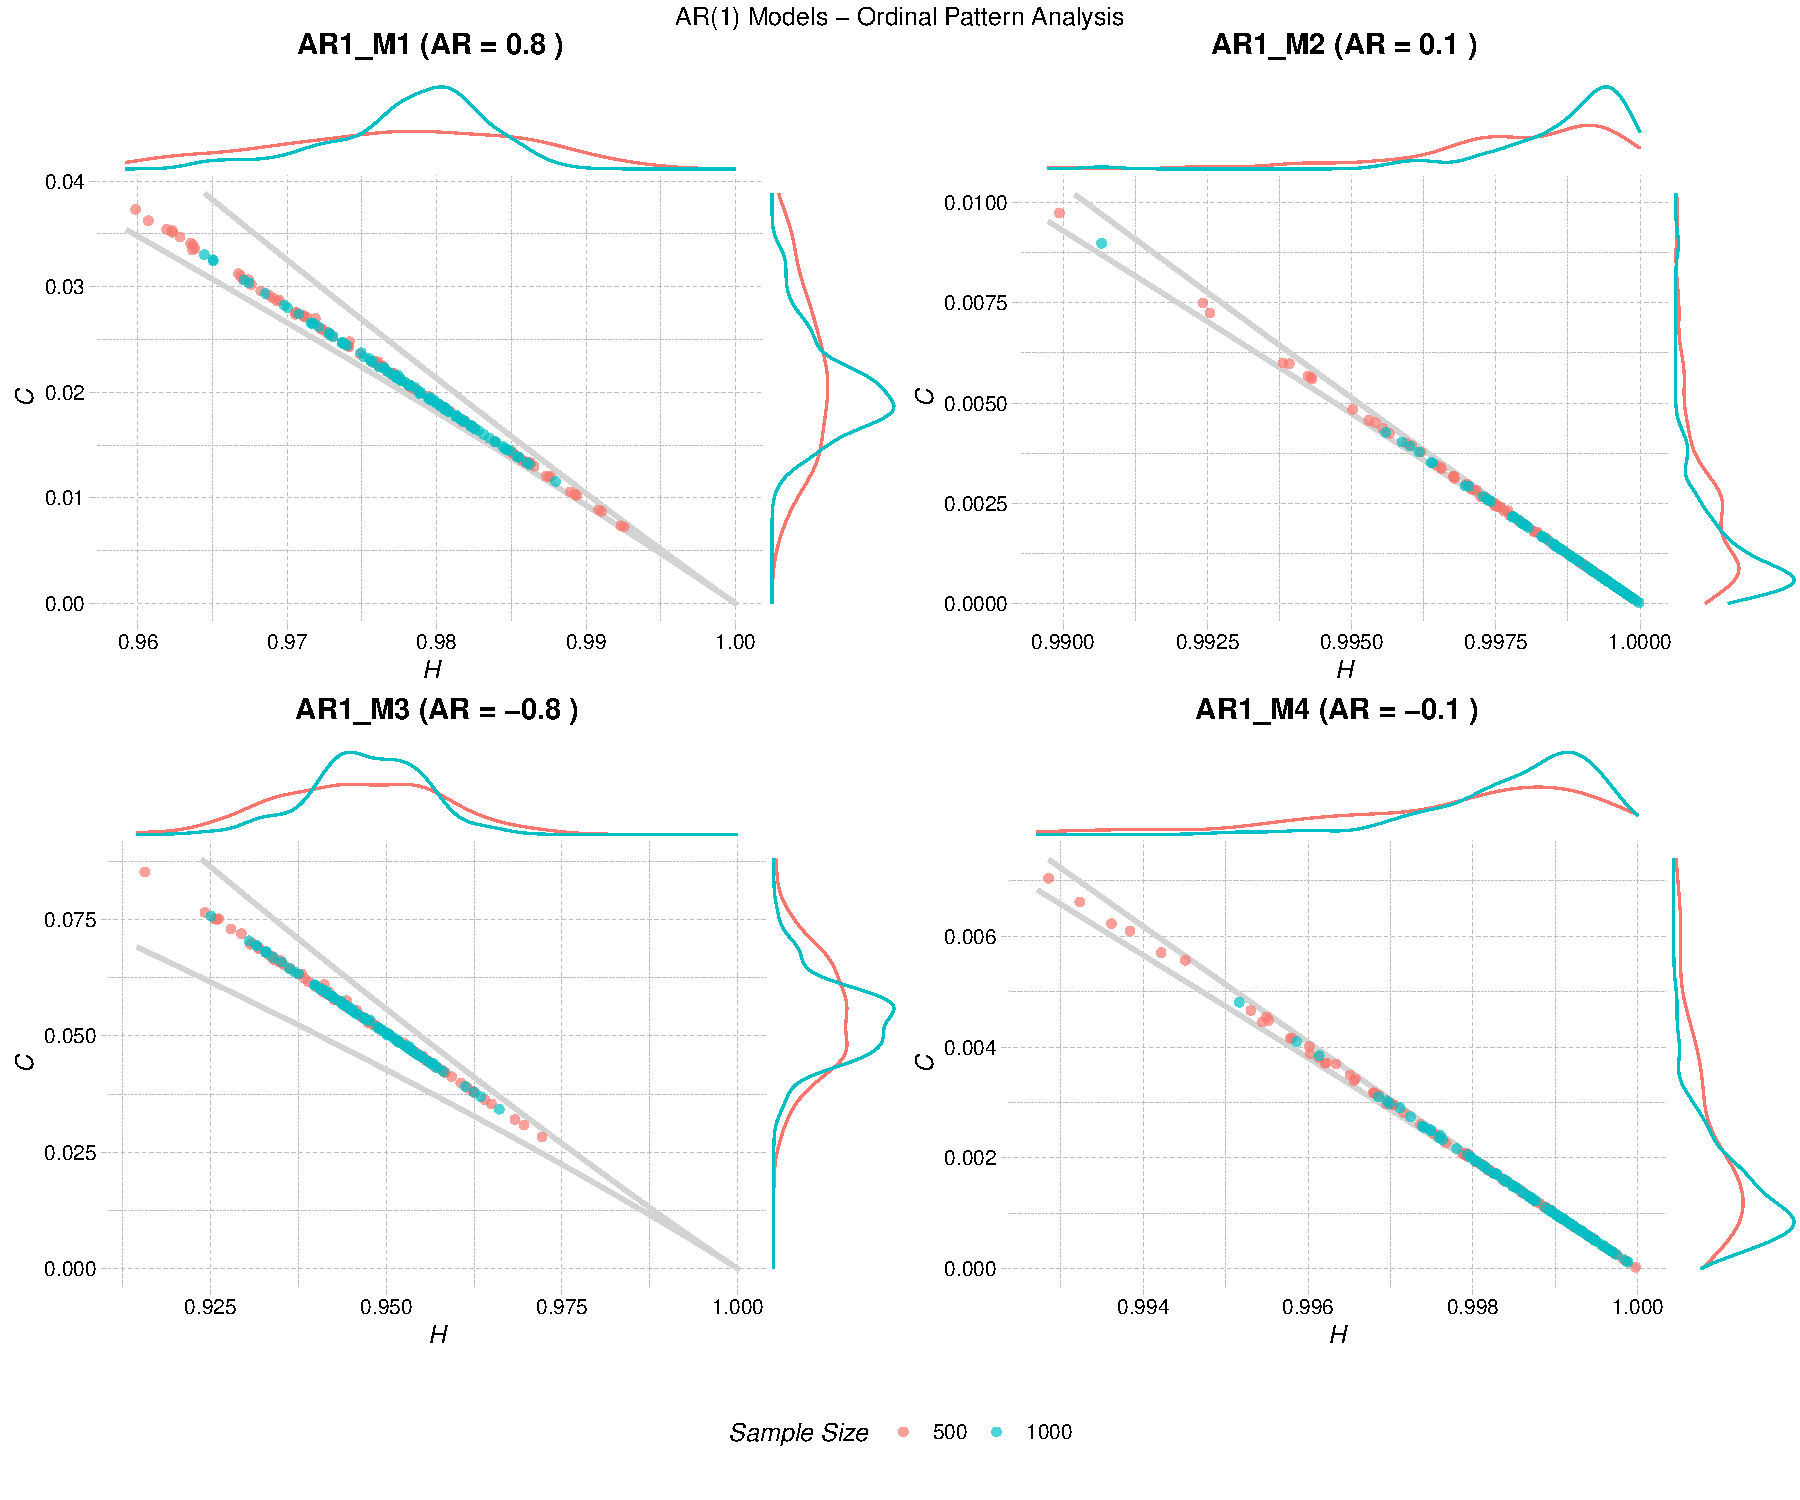
\includegraphics[width=0.9 \textwidth]{AR1_combined_analysis}
%	\caption{$H \times C$ plane for AR(1) model}
%	\label{fig:HC AR(1)}
%\end{figure}	

%\begin{figure}[H]
%	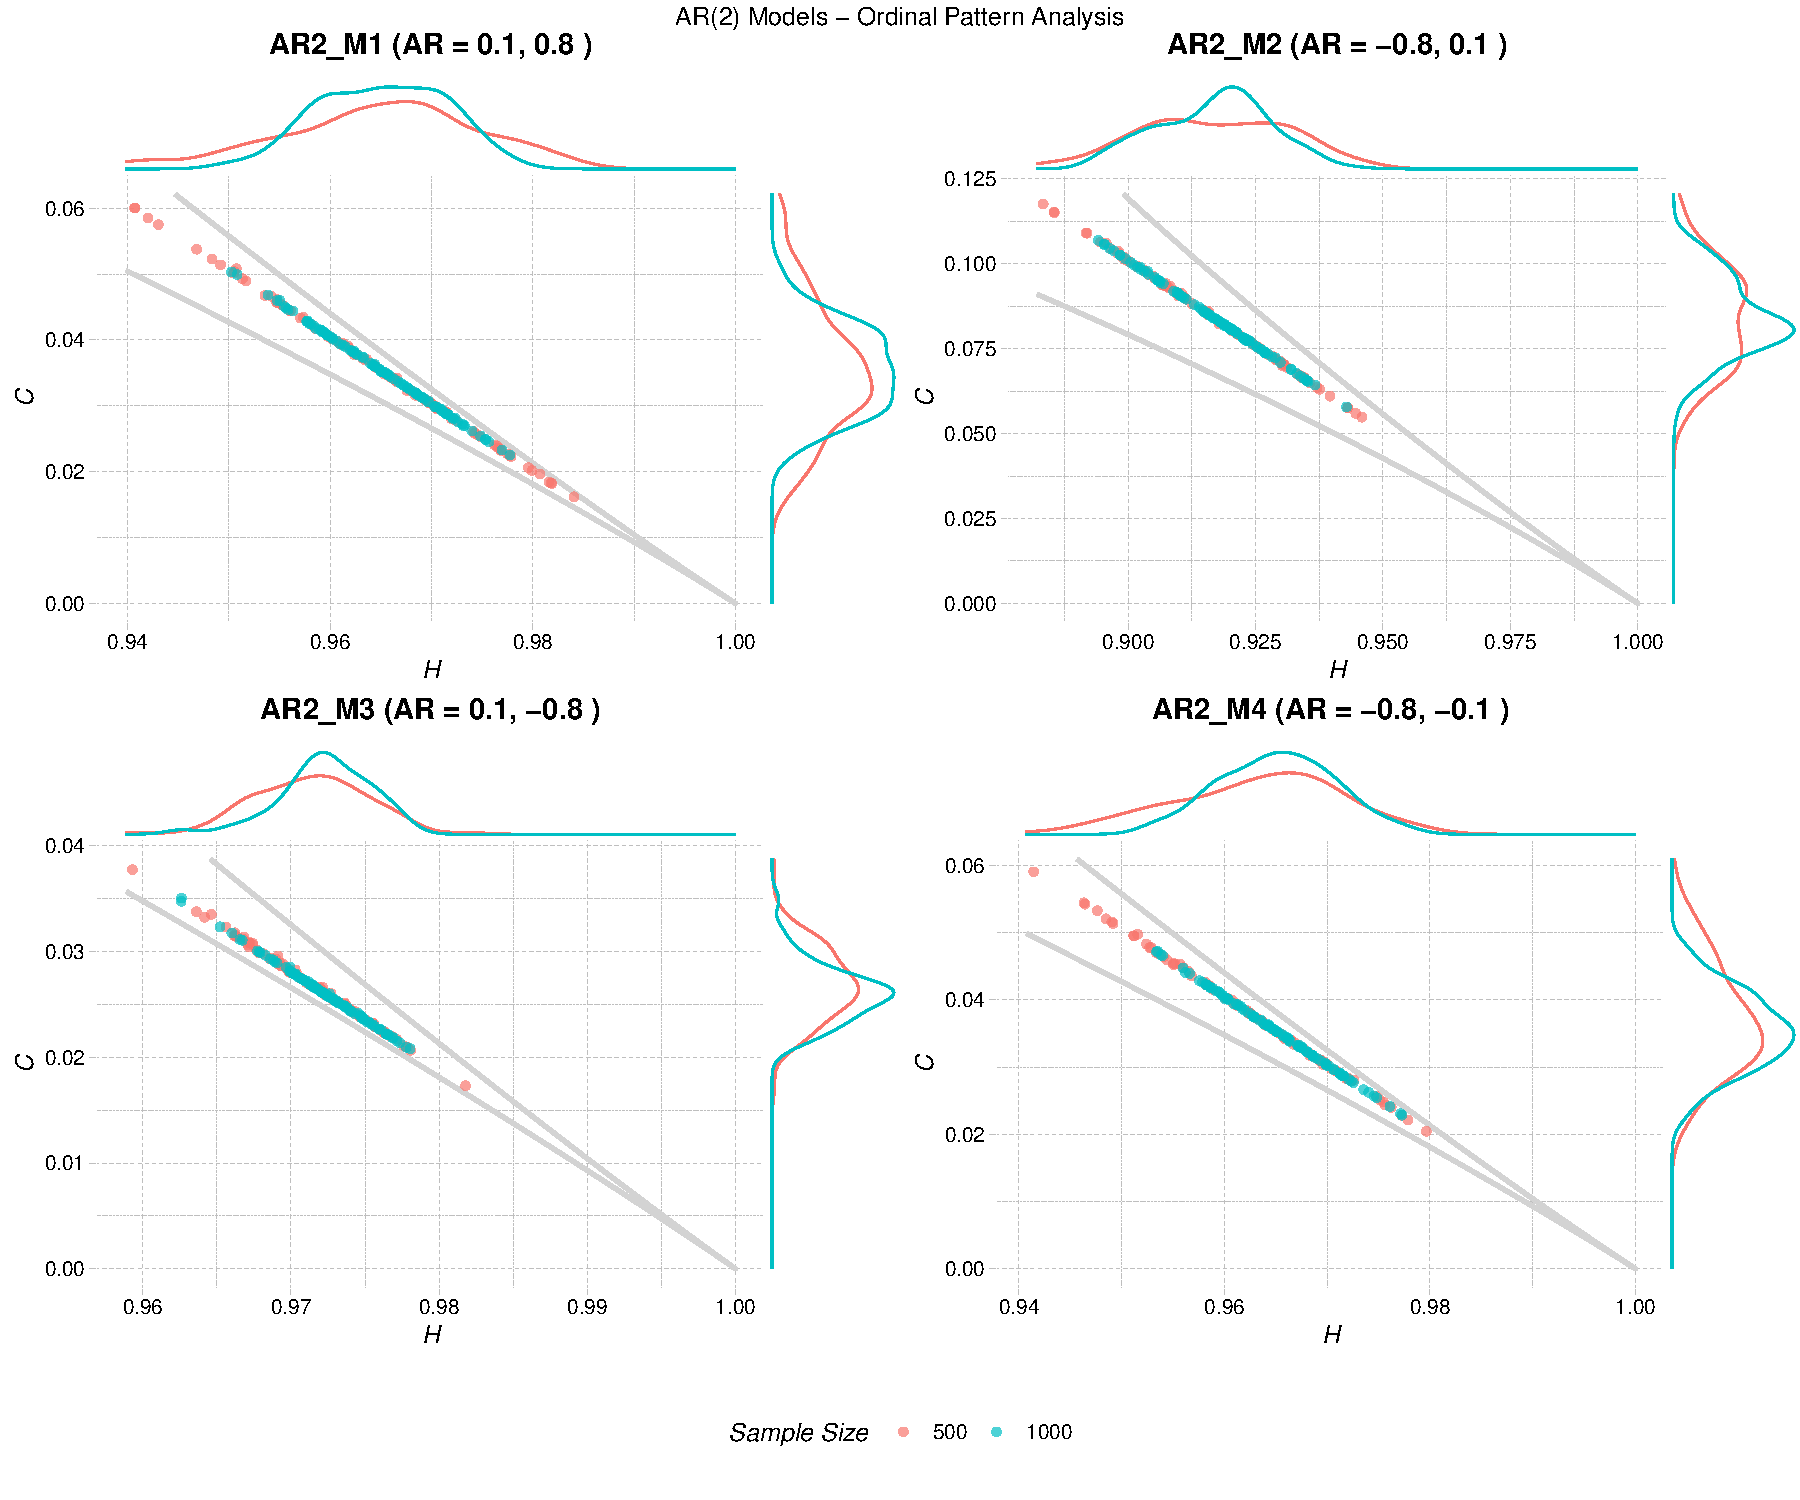
\includegraphics[width=0.9 \textwidth]{AR2_combined_analysis}
%	\caption{$H \times C$ plane for AR(2) model}
%	\label{fig:HC AR(2)}
%\end{figure}

%\begin{figure}[H]
%	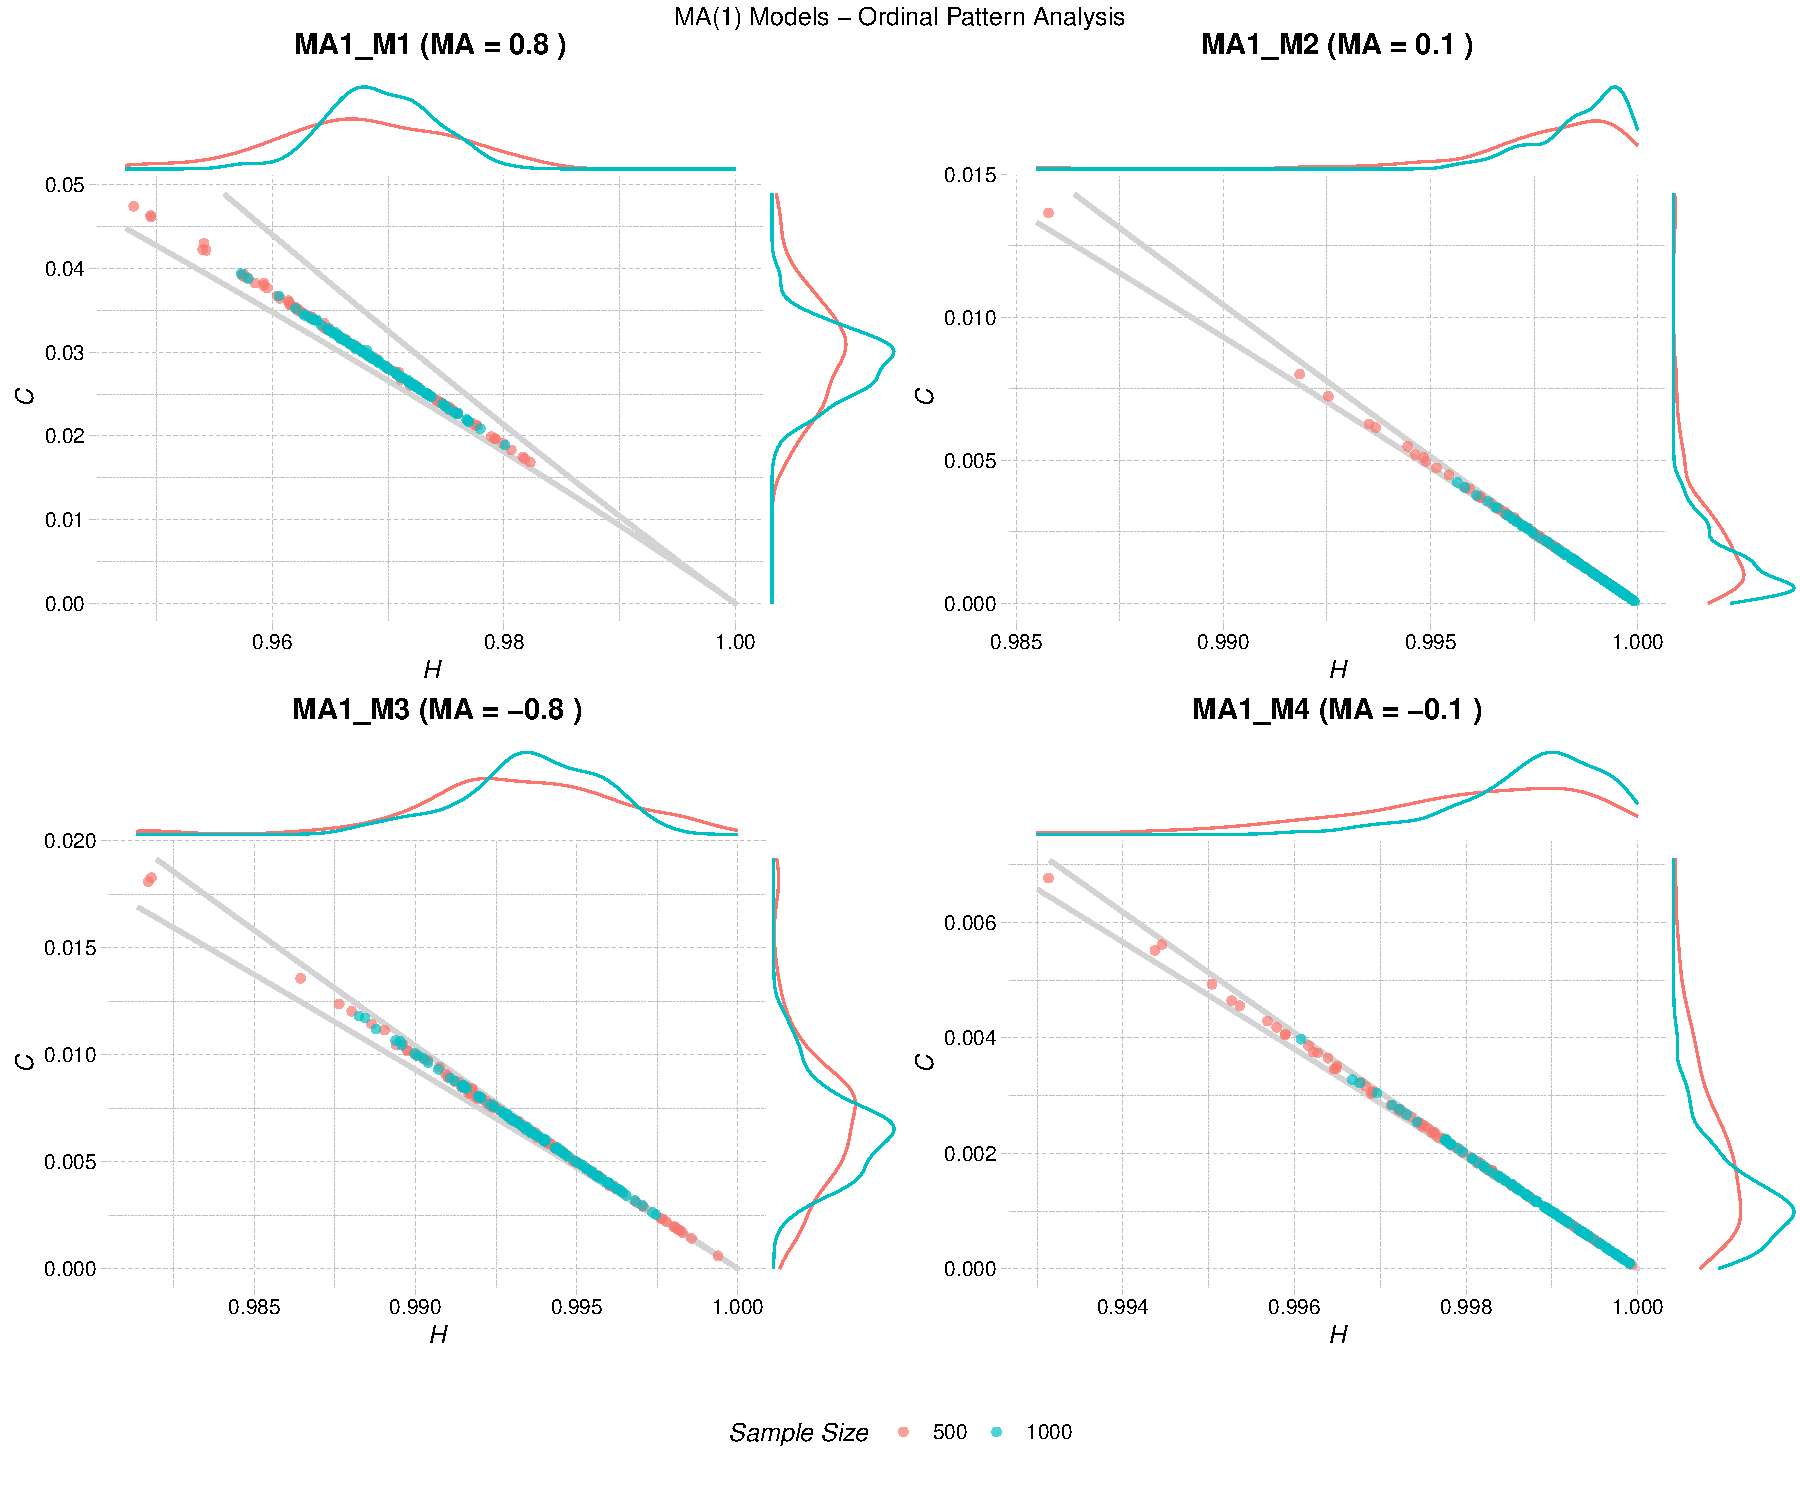
\includegraphics[width=0.9 \textwidth]{MA1_combined_analysis}
%	\caption{$H \times C$ plane for MA(1) model}
%	\label{fig:HC MA(1)}
%\end{figure}

%\begin{figure}[H]
%	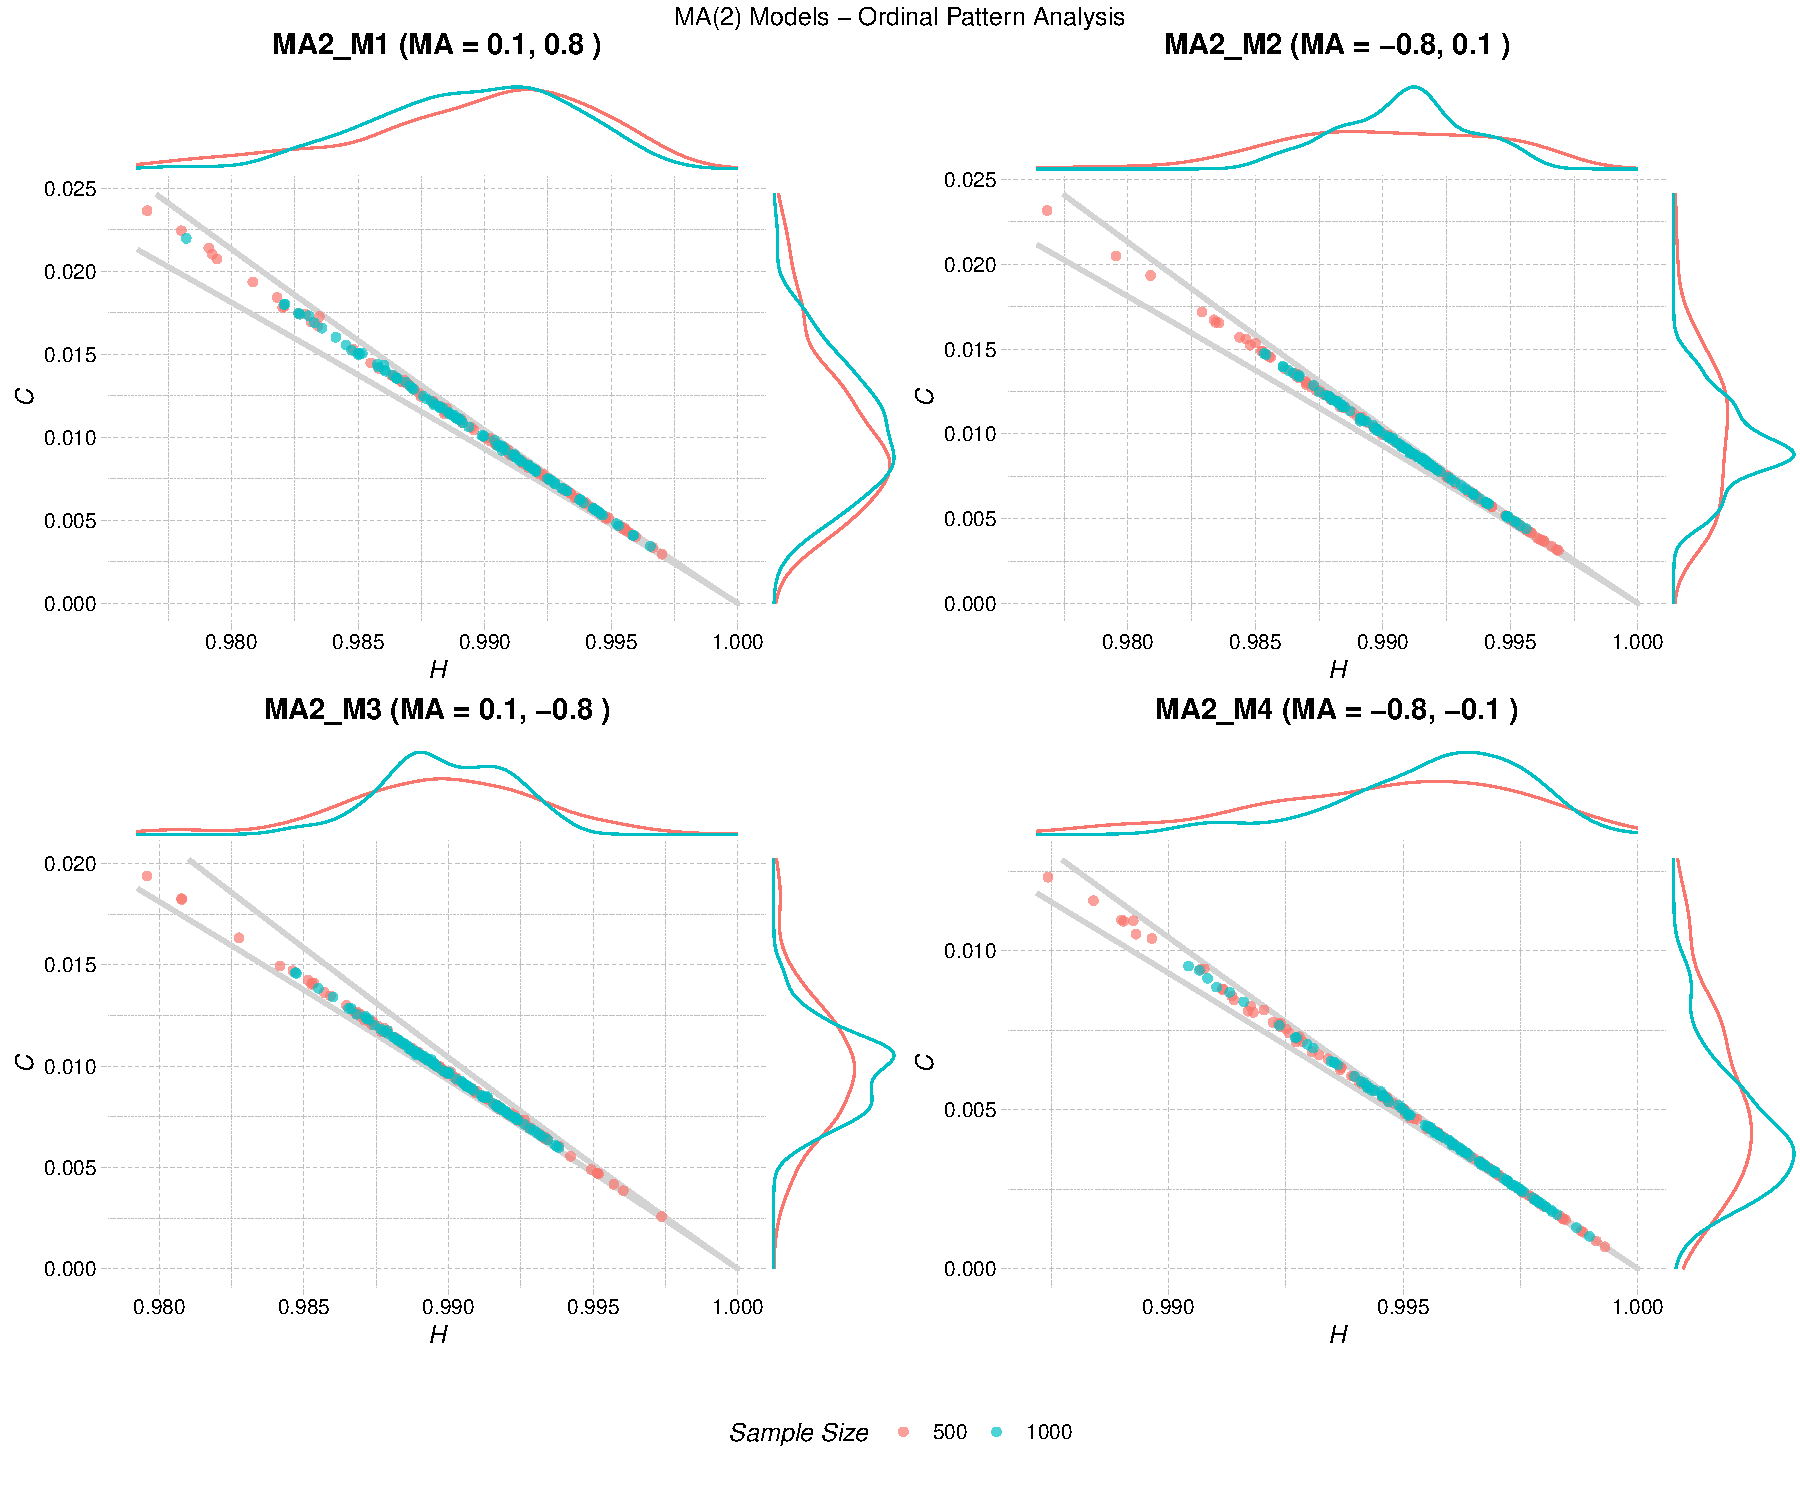
\includegraphics[width=0.9 \textwidth]{MA2_combined_analysis}
%	\caption{$H \times C$ plane for MA(2) model}
%	\label{fig:HC MA(2)}
%\end{figure}			
	
%\begin{figure}[H]
%	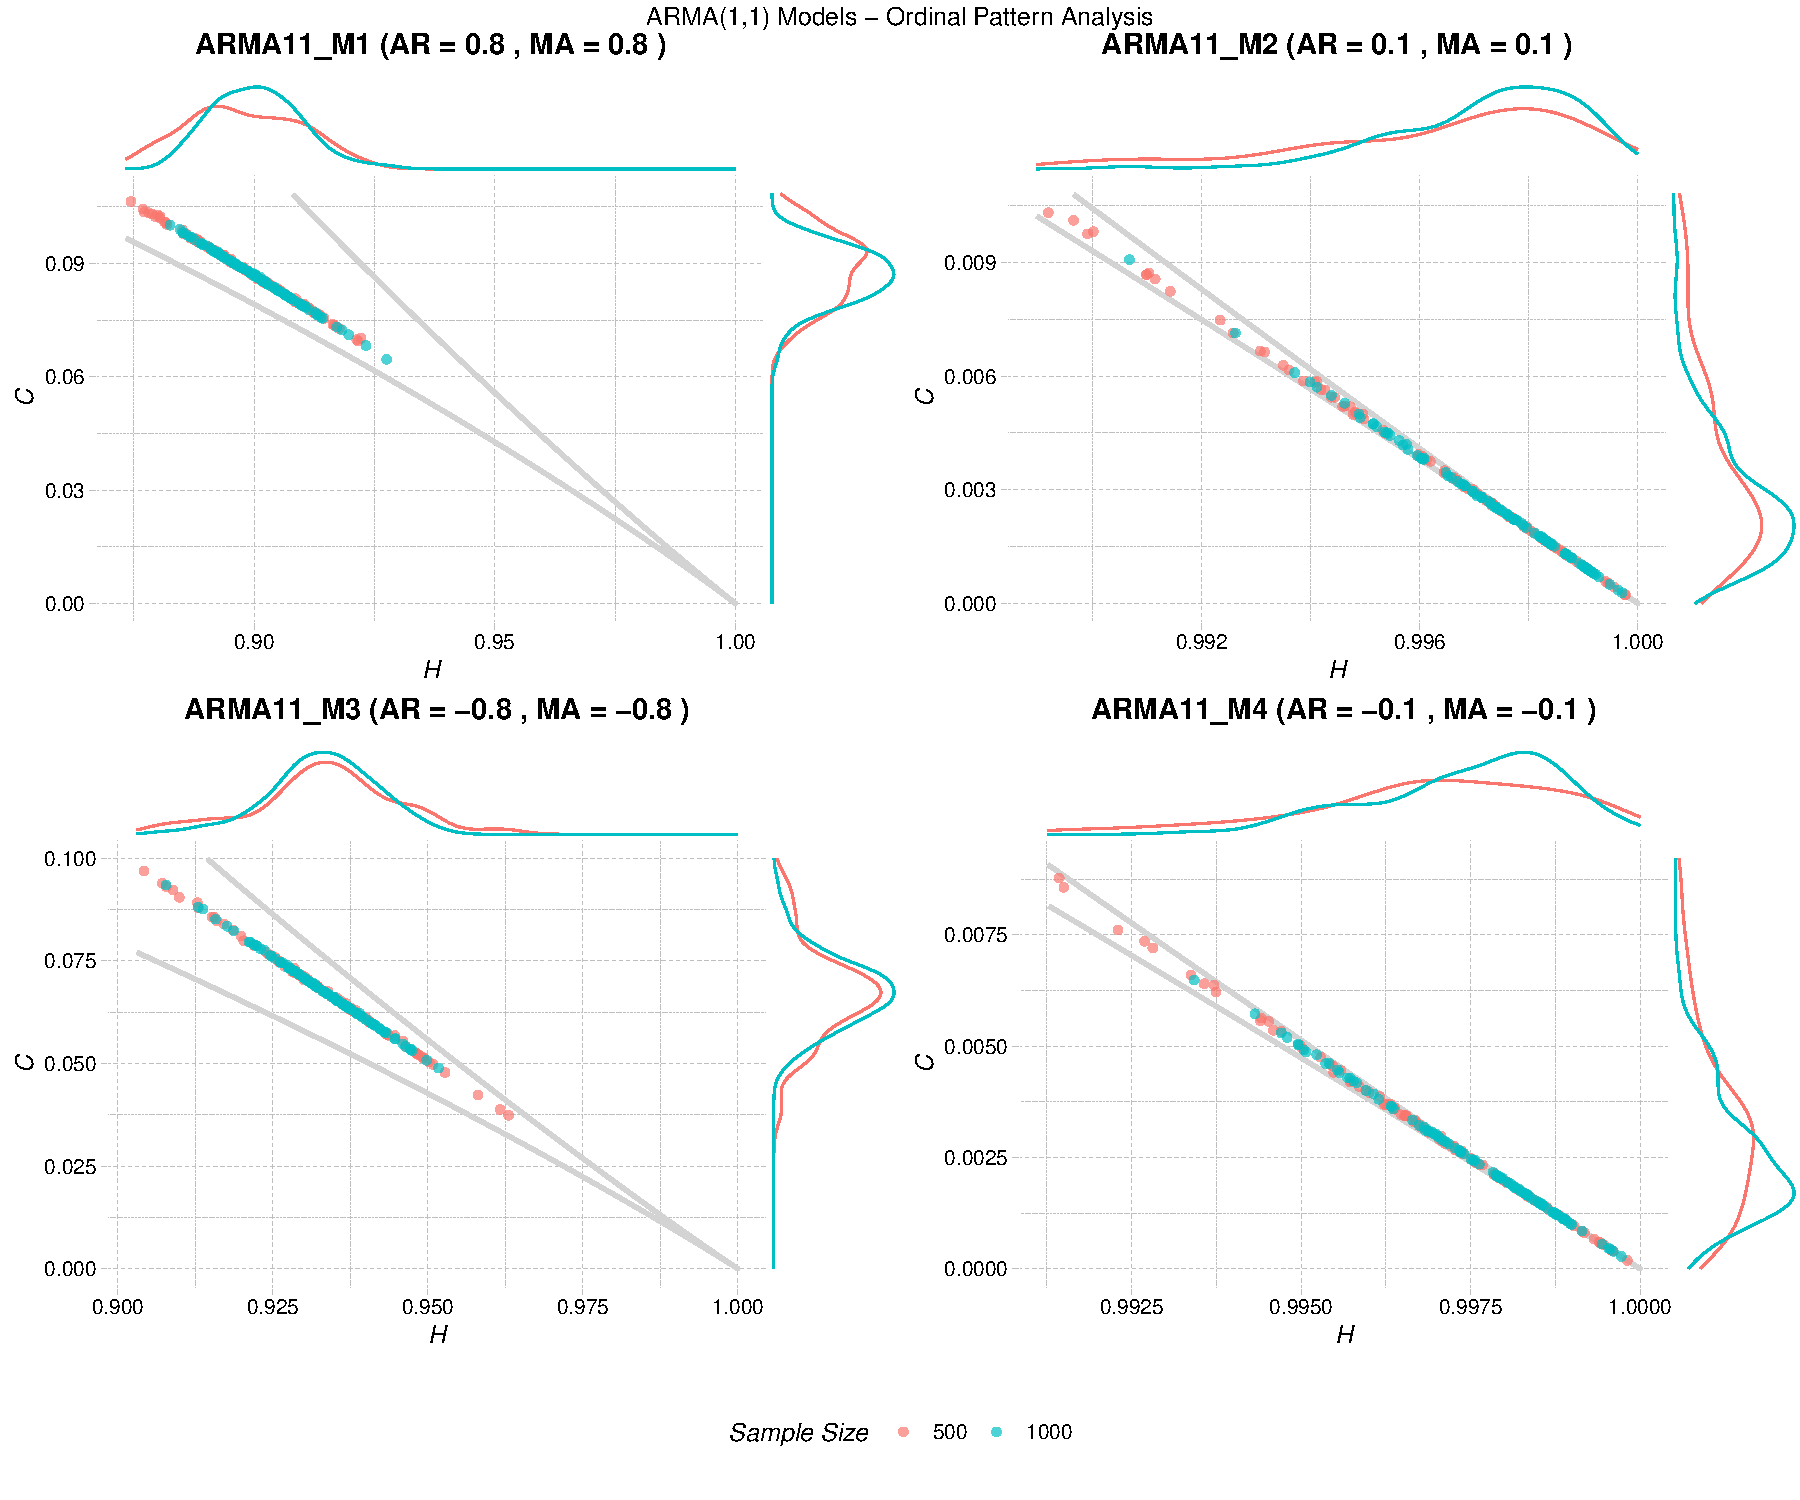
\includegraphics[width=0.9 \textwidth]{ARMA11_combined_analysis}
%	\caption{$H \times C$ plane for ARMA(1,1) model}
%	\label{fig:HC ARMA(11)}
%\end{figure}	

%\begin{figure}[H]
%	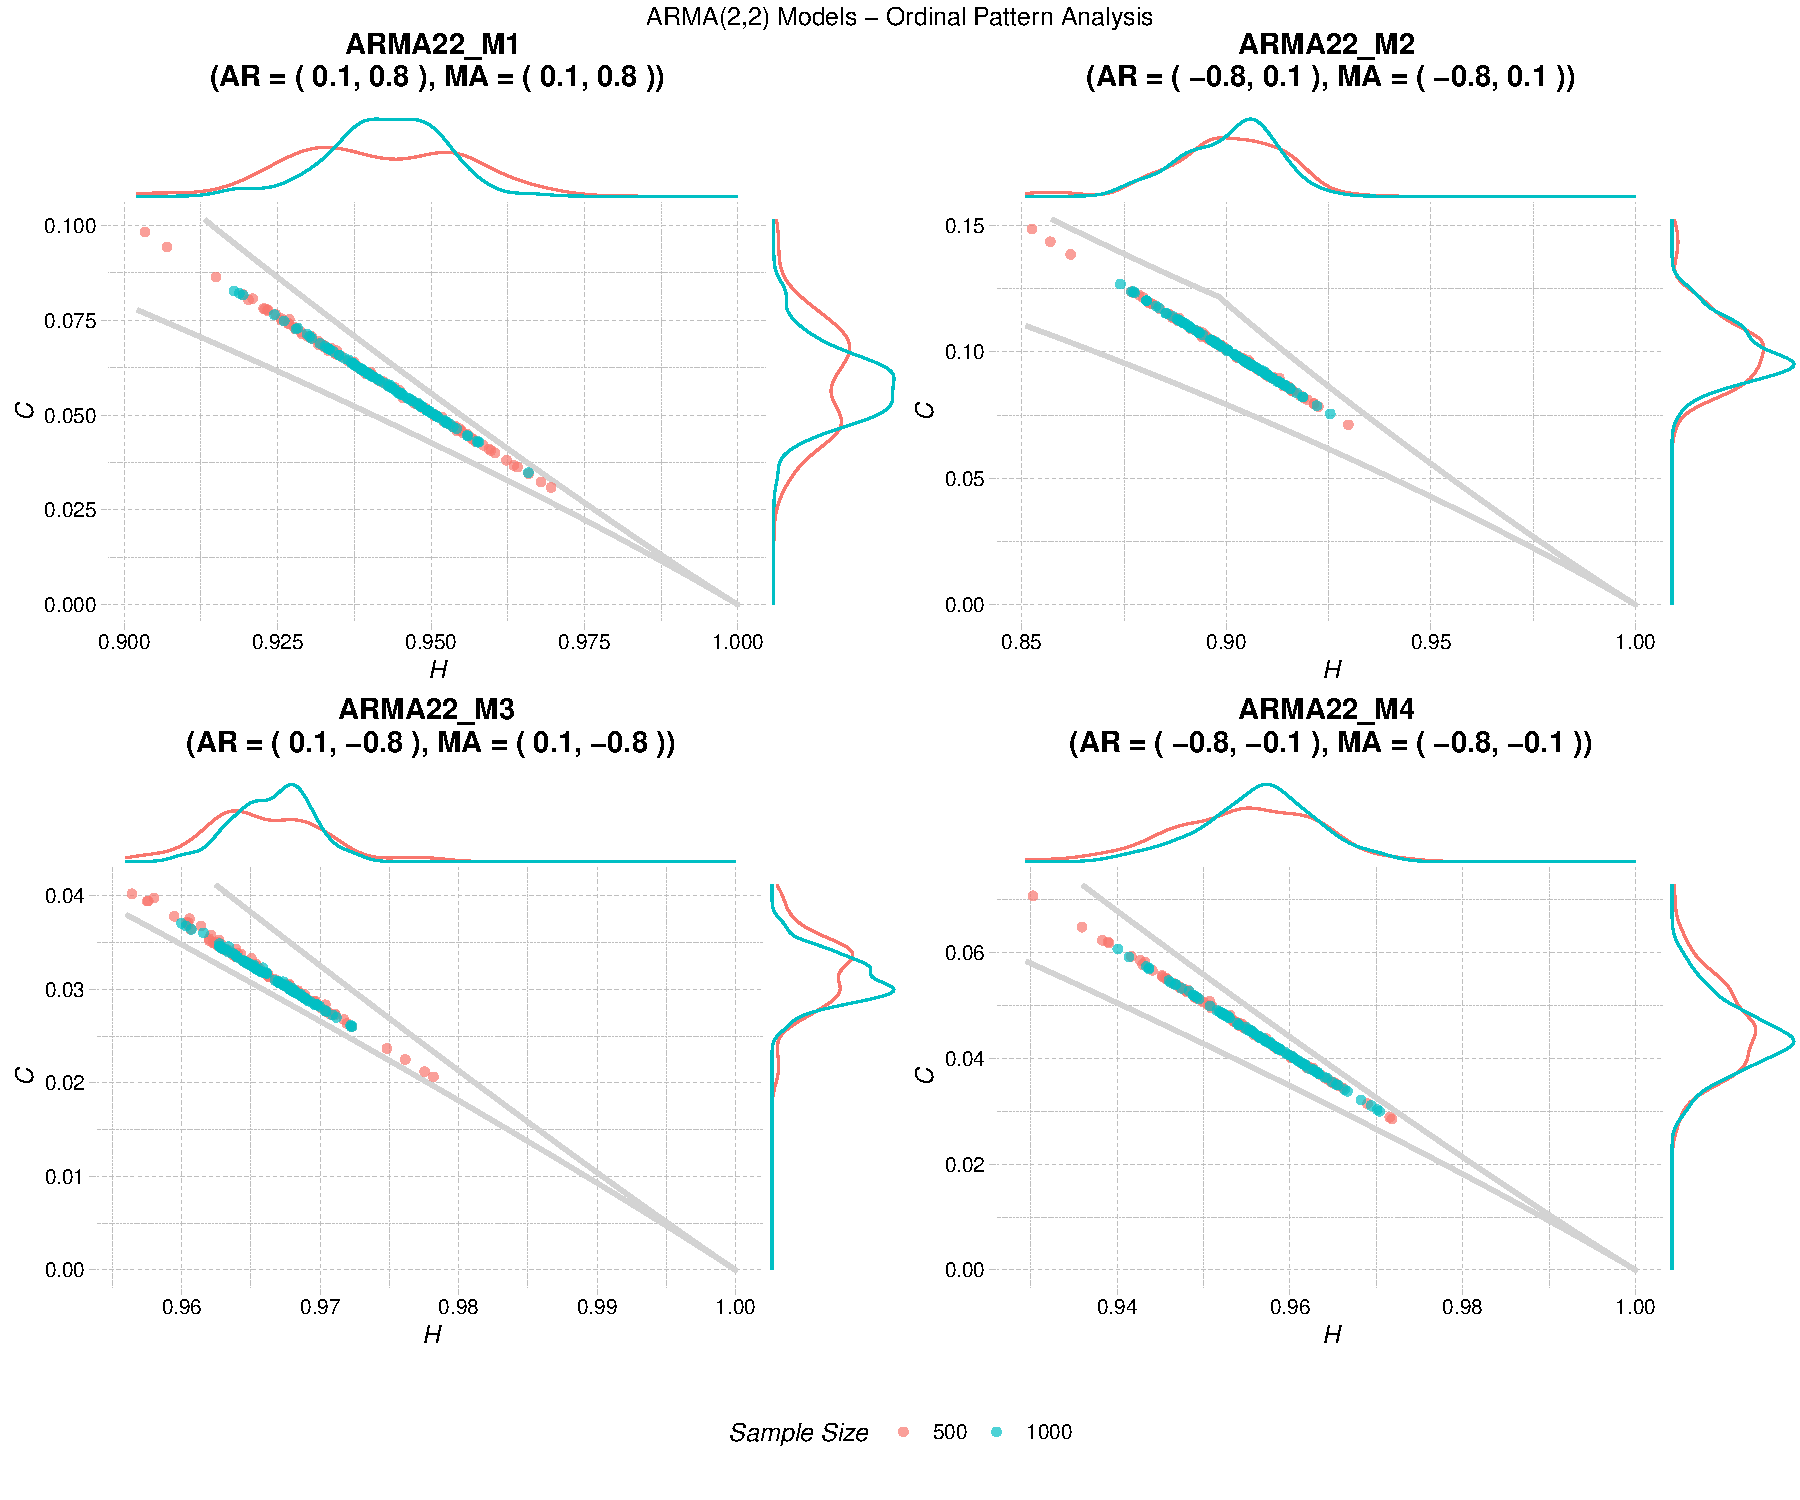
\includegraphics[width=0.9 \textwidth]{ARMA22_combined_analysis}
%	\caption{$H \times C$ plane for ARMA(2,2) model}
%	\label{fig:HC ARMA(22)}
%\end{figure}

Further analysis using advanced clustering validation in the entropy–complexity plane is considered to achieve a more rigorous differentiation and assessment of clustering validity.

For a more detailed investigation of the results, each process type was analyzed separately with respect to the AR, MA, and ARMA model structures. A closer examination of the results, as illustrated in Figure~\ref{fig:HC new n1000}, reveals clear differences among the model classes within the entropy–complexity plane.

%\begin{figure}[H]
%	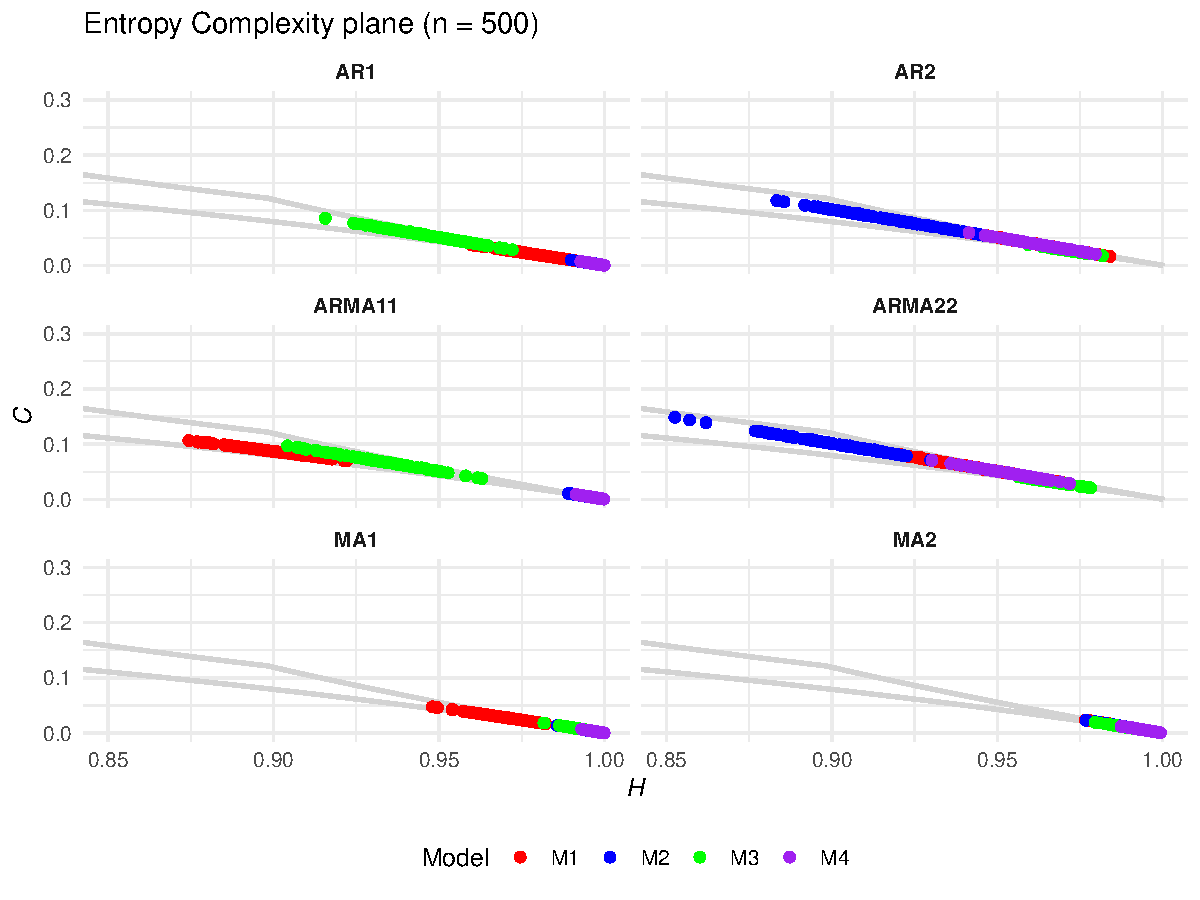
\includegraphics[width=0.9 \textwidth]{New_model_group_plot_n500}
%	\caption{$H \times C$ plane for new model n500}
%	\label{fig:HC new n500}
%\end{figure}

\begin{figure}[H]
	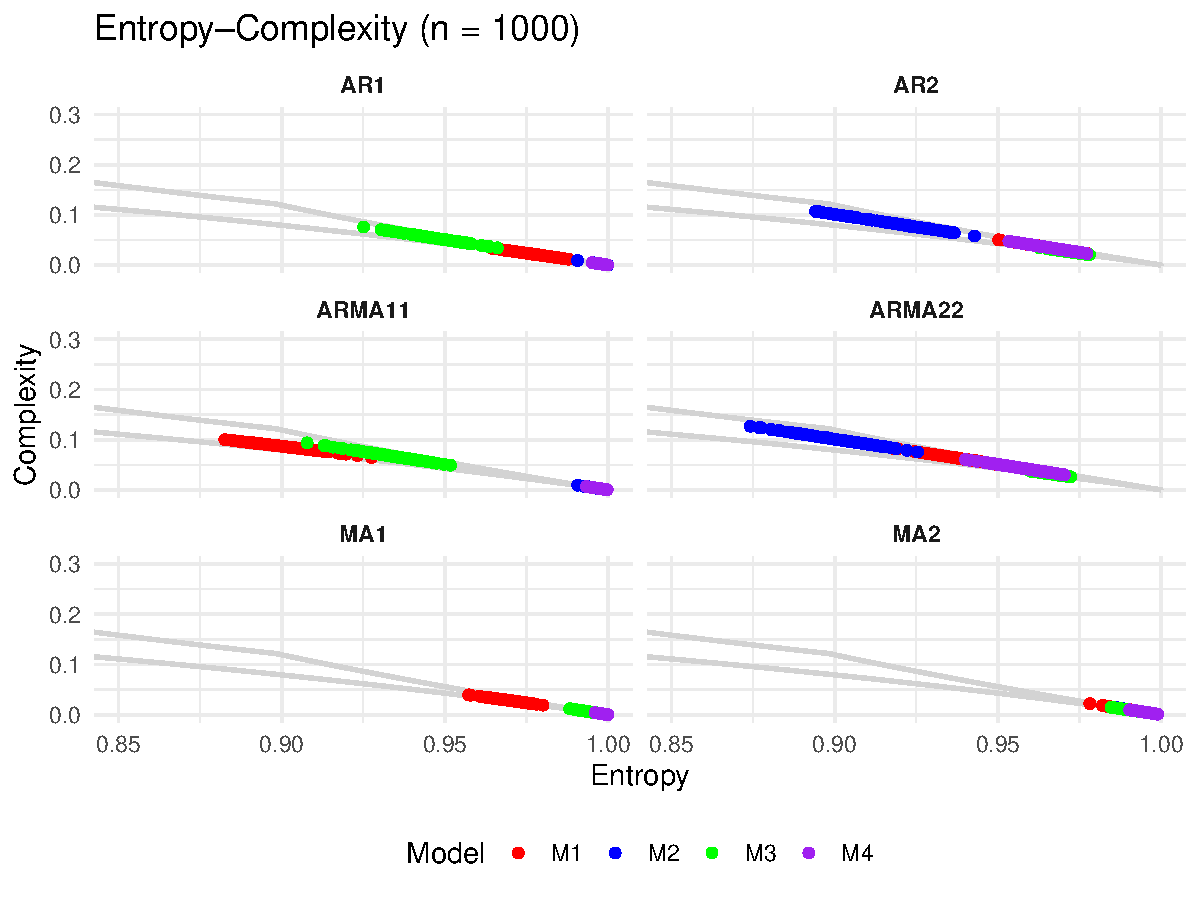
\includegraphics[width=0.9 \textwidth]{New_model_group_plot_n1000}
	\caption{$H \times C$ plane for new model n1000}
	\label{fig:HC new n1000}
\end{figure}

\section{Discussion}
The combination of summary statistics and ordinal pattern clustering allows for robust differentiation among AR, MA, and ARMA models. ARMA models, especially higher order, are distinguishable via their increased variance and entropy-complexity characteristics.

The results from the entropy–complexity analysis across $\mathrm{AR}(1), \mathrm{AR}(2)$, $\mathrm{MA}(1), \mathrm{MA}(2),$ $\mathrm{ARMA}(1,1),$ and $\mathrm{ARMA}(2,2)$ models reveal distinct clustering and spread patterns. These results provide key insights into the structural effects of different time series model classes and parameter variation.

For the$\mathrm{AR}(1)$ models, series with stronger positive or negative coefficients exhibit lower entropy and higher complexity. In contrast, smaller coefficients allow greater entropy variation. 

$\mathrm{AR}(2)$ models produce a wider spread in the entropy–complexity plane. This reflects the richer dynamics possible with two autoregressive lags. However, stationary parameter values remain within a consistent range of complexity.

The $\mathrm{MA}(1)$ and $\mathrm{MA}(2)$ analyses further demonstrate that moving average structure drives most realizations toward lower complexity. Entropy is also tightly controlled, especially for stronger coefficients. It shows that moving averages make data smoother but also shorten how long past values affect the present.

The $\mathrm{ARMA}(1,1)$  and $\mathrm{ARMA}(2,2)$ joint models combine these mechanisms. As a result, they produce denser, but still distinct, groupings in the ($H \times C$) diagram as both AR and MA parameters interact.

\section{Conclusion}
Summary statistics and time series plots provide initial model discrimination. Ordinal pattern clustering (entropy-complexity plane) strongly supports identification and categorization of AR, MA, and ARMA model dynamics.

Overall, this analysis shows how model order and parameter values directly influence the diversity and location of points in the entropy–complexity plane. These results support the use of entropy and complexity for both identification and clustering of time series dynamics.



	
%	\bibliography{../BearingFaultDiagnosis}
	
\end{document}

